\section{Wykorzystane technologie}
\label{cha:technologie}

\subsection{Ontologia}
\label{sec:ont}

Ontologia jest formalną reprezentacją pewnej dziedziny wiedzy. Składają się na nią zapis zbiorów pojęć i relacji między nimi. Zapis ten tworzy schemat pojęciowy, który jest opisem danej dziedziny wiedzy. Może służyć jednocześnie jako podstawa do wnioskowania o właściwości opisywanych ontologią pojęć.	 \cite {7}

Pod pojęciem ontologii mogą się kryć różne struktury wiedzy. Ich przeznaczenie czy zakres stosowania może być wieloraki.

Ontologie możemy podzielić ze względu na stopień ich formalizacji:
\begin{itemize}
\item nieformalne
	\begin{itemize}
		\item predefiniowane słownictow
		\item słowniki
		\item tezarusy
		\item taksonomie
	\end{itemize}
\item formalne
	\begin{itemize}
		\item ontologie oparte na danych
		\item ontologie oparte na logice
	\end{itemize}
\end{itemize}

Podział następuje także ze względu na zakres stosowania:
\begin{itemize}
\item ontologie wysokiego poziomu (\textit{upper ontologies})
\item ontologie dziedzinowe (\textit{domain ontologies})
\item ontologie aplikacyjne
\end{itemize}

Istnieje szereg języków pozwalających na zapis lub wspierających ontologie:
\begin{itemize}
\item OWL (\textit{Ontology Web Language})
\item RDF (\textit{Resource Description Framework})
\item RDF Vocabulary Description Language (RDF Schema, RDFS)
\item OCML (Operational Conceptual Modeling Language)
\item XML (Extensible Markup Language)
\end{itemize}

\subsection{OWL}
\label{sec:owl}

OWL (Ontology Web Language) jest opartym na składni XML językiem służącym do opisu ontologii. Stanowi on rozszerzenie języka RDF (Resource Definition Language). Istnieją 3 odmiany OWL: OWL Lite, OWL DL oraz OWL Full. W 2004 roku język ten został uznany za standard przez organizację W3C. \cite {8}

OWL został stworzony do przetwarzania informacji o obiektach oraz relacji między nimi, nie do przechowywania tych informacji w formie czytelnej dla człowieka. OWL jest zbudowany na bazie RDF, tak więc języki te są ze sobą w pełni kompatybilne. OWL posiada jednak znacznie mocniejszą składnię.

Do elementów języka OWL należą takie atrybuty jak:

\begin{itemize}

\item Class - definiuje grupę indywidualnosci, które posiadają pewne wspólne cechy. Klasy można organizować w hierarchie za pomocą atrybutu subClassOf.


\item rdf:Property - okresla pewne relacje między indywidualnosciami np. samochod może posiadać drzwi, osoba moze posiadać dziecko albo rodzica.

\item rdfs:domain - ogranicza indywidualności, do których można zastosować relację (property). Jeżeli relacja łączy jedną indywidualność z drugą, i jednocześnie posiada ona domenę na określoną klasę, to obie indywidualności muszą należeć do tej klasy.

\item rdfs:range - ogranicza nie tylko indywidualności, ale także wartość relacji (property)

\item Individual - indywidualności są instancjami klas, które są połączone pewnymi relacjami (property).

\end{itemize}

Wszystkie powyższe atrybuty są częścią specyfikacji OWL Lite.

\subsection{Protege}
\label{sec:protege}
Protege jest otwarto-źródłowym narzędziem stworzonym przez Stanford Medical Informatics \cite{26}. Jak przy większości narzędzi modelujących, architektura Protege jest przejrzyście podzielona na dwie części - model i widok. Modele są wewnętrzną reprezentacją mechanizmy ontologii i baz wiedzy. Widoki zapewniają interfejs użytkownika, dzięki któremu można wyświetlać i manipulować modelami.

Protege posiada możliwość wczytania, edycji i zapisywania w wielu popularnych dla ontologii formatach, np:
\begin{itemize}
\item RDF
\item OWL
\item XML
\item UML
\item Bazy relacyjne
\end{itemize}

\subsection{SPARQL}
\label{sec:sparql}

~SPARQL jest językiem zapytań RDF, czyli pozwala na wyciaganie lub manipulowanie danymi w bazie danych składującej dane w formacie RDF (eng. Resource Description Framework). SPARQL pozwala również na pracę na danych w formacie pochodnym od formatu RDF, np. OWL, jednak z pewnymi ograniczeniami. SPARQL operując na danych w formacie OWL musi pominąć elementy języka które nie mają przełożenia na format RDF.

~Konstrukcja zapytań opiera się o zestaw trzech parametrów:
\begin{itemize}
\item spójnika (eng. conjuction)
\item alternatywy (eng. disjunction)
\item wzorzec (opcjonalnie) (eng. pattern)
\end{itemize}

Idea jaka przyświecała twórcom SPARQL określała go jako przełom w tworzeniu internetu czytelnego dla maszyn. Jeżeli format ten przyjmie się jako standard otrzymamy uniwersalny sposób otrzymywania informacji z internetowych \quotedblbase skupisk\textquotedblright  danych, co da nowe możliwości łączenia danych z różnych źródeł.


\subsection{REST}
\label{sec:rest}

REST jest protokołem komunikacji między aplikacjami, który tak naprawdę jest tylko pewną dodatkową warstwą nałożoną na protokół HTTP. Budowanie zapytań restowych z poziomu języków programowania jest tak samo proste, jak zrozumienie działania protokołu HTTP. Istnieje wiele bibliotek i prostych frameworków do budowania serwisów, odbierających i wysyłających zapytania HTTP. Należą do nich np Jersey-RS, czy zbudowana na jego bazie trochę większa biblioteka Apache CXF. Biblioteka Fuserki, będąca częścią specyfikacji Apache Jena oferuje możliwość transferu danych właśnie protokołem REST, przy użyciu języka zapytań SPAQRL.  \cite{1}

Ze względu na swoją prostotę i oparcie o standard HTTP, wybór tego protokołu jako sposobu komunikacji między aplikacjami jest bardzo dobrą decyzją. Umożliwia to znakomitą skalowalność naszego systemu, poprzez rozdzielenie go na szereg indywidualnych aplikacji, które nie muszą być napisane przy użyciu tej samej technologii, muszą jedynie współdzielić tą metodę komunikacji oraz ewentualnie sposób serializacji danych.

\subsection{Fuseki}
\label{sec:rest}

~Fuseki jest to serwer HTTP w standardzie REST przyjmujący zapytania HTTP zawierające w parametrach zapytania SPARQL.
Dzięki niemu możemu w ustandaryzowany sposób pobierać lub manipulowac danymi w modelu OWL lub RDF.

~Fuseki jest jednym z subsystemów systemu Jena. Twórcy zadbali o to żeby serwer SPARQL udało się włączyć nie tylko poprzez konsole, ale również bezpośrednio z aplikacji JAVA z wykorzystaniem biblioteki Jena.

\subsection{HL7}
\label{sec:hl7}

HL7 (Health Level 7) jest organizacją ustanawiającą standardy, akredytowaną przez American National Standards Insitute (ANSI). Opracowali protokół komunikacyjny szeroko używany w USA, obecnie coraz częściej rozpoznawany i wykorzystywany w pozostałych częściach świata. \cite {14}

RIM (Reference Informational Model) został wykorzystany w trzeciej wersji HL7 (HL7 Version 3) w celu standaryzacji powiązań pomiędzy danymi przenoszonymi przez wiadomości protokołu HL7. \cite {16}

Diagram UML na rysunku \ref{fig:hl7rim} przedstawia podstawowe klasy istniejące w RIM. \cite {15}

RIM opiera się na pięciu podstawowych założeniach:
\begin{itemize}
	\item Każde zdarzenie jest opisane przez klasę Act
	\begin{itemize}
		\item zdarzeniem może być: procedura, obserwacja, dostawa zapasów, rejestracja, itp.
	\end{itemize}
 	\item Relacje pomiędzy zdarzeniami opisuje klasa ActRelationship
 	\item Klasa Participation definiuje kontekst wystąpienia zdarzenia
 	\begin{itemize}
 		\item autor, wykonujący, podmiot, lokalizacja itp.
 	\end{itemize}
 	\item uczestnicy zdarzenia są opisanie przez klasę Role
 	\begin{itemize}
 		\item pacjent, dostawca, praktykant, pracownik itp.
 	\end{itemize}
  	\item role są reprezentowane przez klasę Entity
  	\begin{itemize}
 		\item osoby, organizacja, materiały, miejsca, urządzenia, itp.
 	\end{itemize}
\end{itemize}

\end{multicols}
\begin{figure}[h]
	\center
	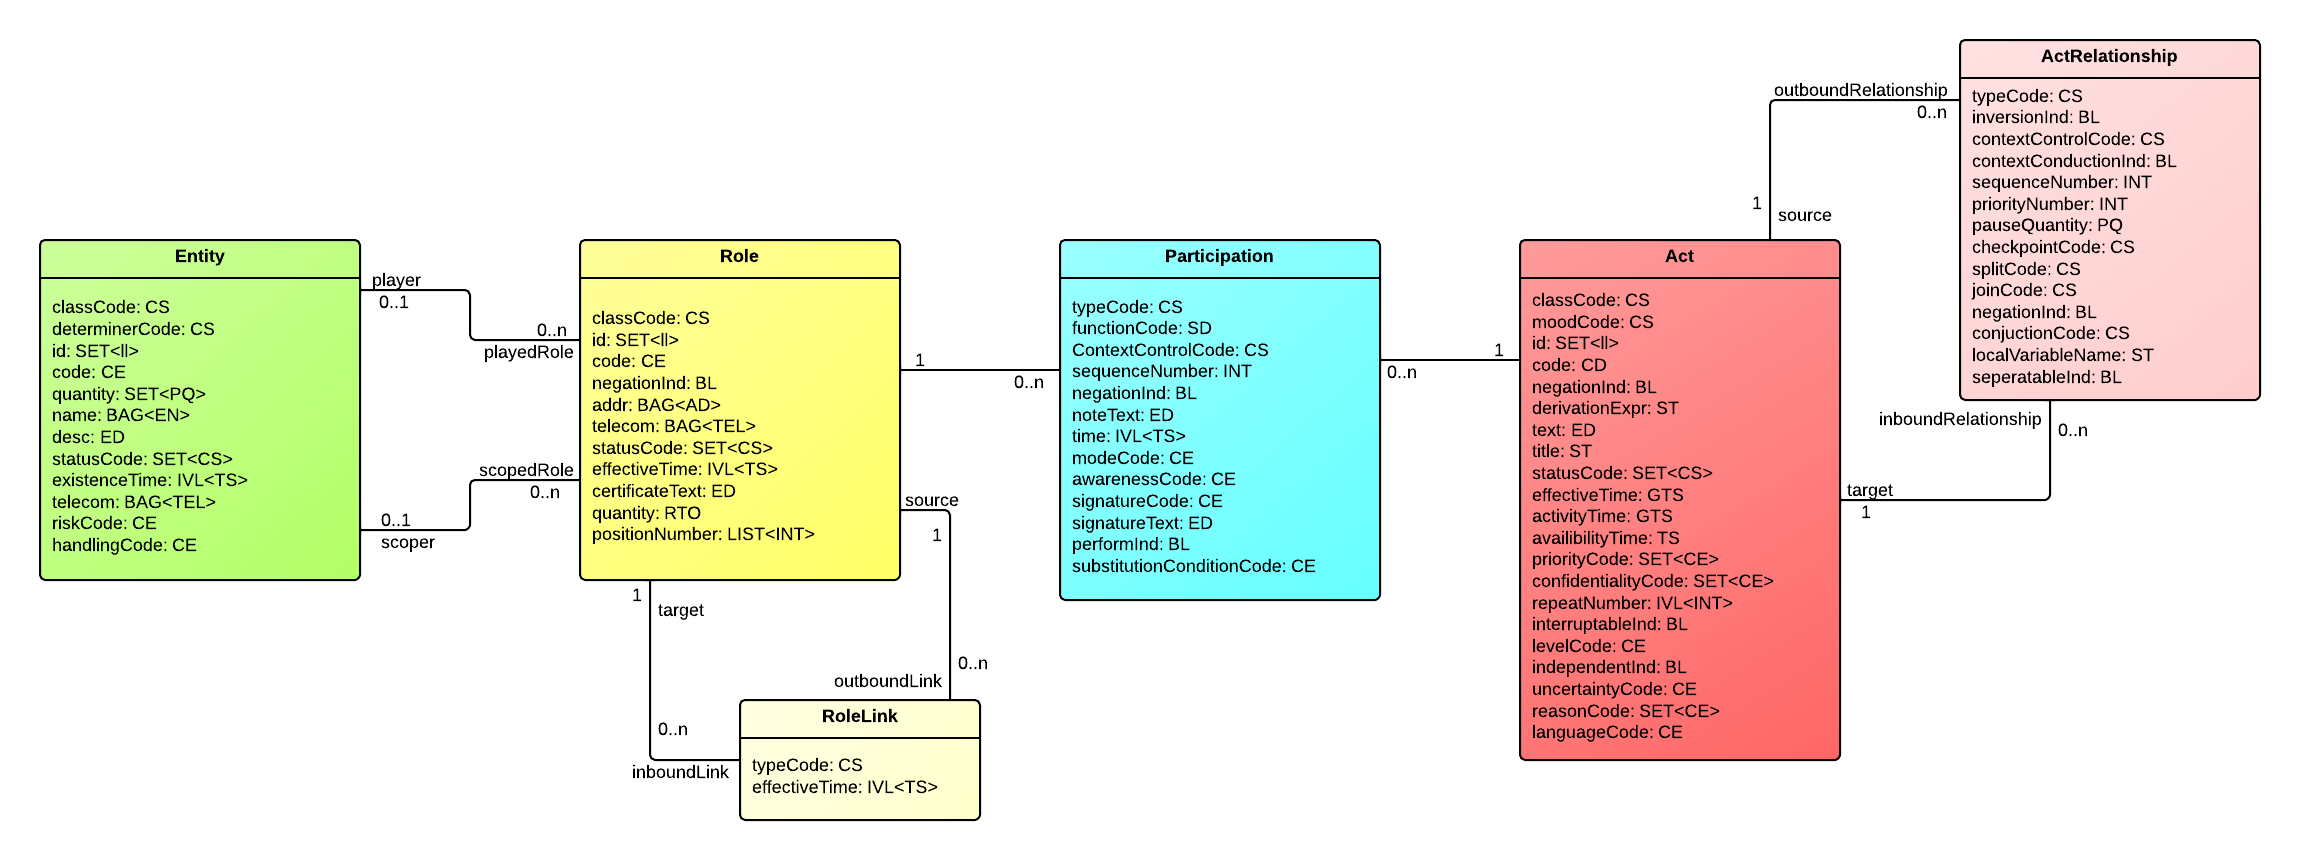
\includegraphics[width=\textwidth, scale=0.5]{pics/HL7}
	\caption{HL7 RIM}
	\label{fig:hl7rim}
\end{figure}
\begin{multicols}{2}